\section{Chart::Lines}
\herv{Name:} Chart::Lines\\ \\
\herv{File:} Lines.pm\\ \\
\herv{Requires:}Chart::Base, GD, Carp, FileHandle\\ \\
\herv{Description:} \fett{Lines} is a \fett{subclass} of Chart::Base.\\
The class Lines creates a lines chart.\\
\\
\herv{Example:}
\begin{figure}[h]
	\begin{center}
		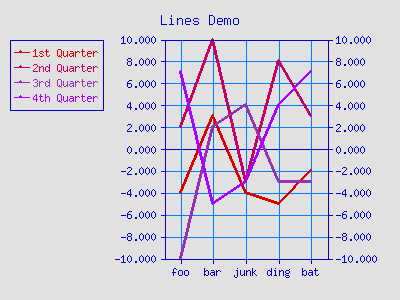
\includegraphics[scale=0.5]{d_lines2.png}
	\end{center}
	\caption{Lines chart}
	\label{fig:lines}
\end{figure}
\begin{verbatim}
use Chart::Lines;

$g = Chart::Lines->new();
$g->add_dataset ('foo', 'bar', 'junk', 'ding', 'bat');
$g->add_dataset ( -4,  3, -4, -5, -2);
$g->add_dataset (  2, 10, -3,  8,  3);
$g->add_dataset (-10,  2,  4, -3, -3);
$g->add_dataset (  7, -5, -3,  4,  7);

%hash = ('legend_labels' => ['1st Quarter', '2nd Quarter',
                             '3rd Quarter', '4th Quarter'],
         'y_axes' => 'both',
         'title' => 'Lines Demo',
         'grid_lines' => 'true',
         'legend' => 'left',
         'legend_example_size' => 20,
         'colors' => {'text' => 'blue',
                      'misc' => 'blue',
                      'background' => 'grey',
                      'grid_lines' => 'light_blue',
                      'dataset0' => [220,0,0],
                      'dataset1' => [200,0,100],
                      'dataset2' => [150,50,175],
                      'dataset3' => [170,0,255] },
         );

$g->set (%hash);

$g->png ("lines.png");
\end{verbatim}
\herv{Constructor:} An instance of a lines chart object can be created with the constructor new():\\
\fett{\$obj = Chart::Lines->new();}\\
\fett{\$obj = Chart::Lines->new(\kursiv{width}, \kursiv{height});}\\
\\
If \fett{new} has no arguments, the constructor returns an image with the size 300x400 pixels. If new has two arguments \kursiv{width} and \kursiv{height}, it returns an image with the desired size. \\ 
\\ 
\herv{Methods:}All universally valid methods, see page \pageref{methods}: Chart::Base. \\
\\
\herv{Attributes/Options:} All universally valid options, see page \pageref{options}. Special options for this type of chart are:\\
\begin{description}
\item['y\_axes'] Tells chart where to place the y-axis. Valid values are 'left', 'right' and 'both'. Defaults to 'left'.
\item['brush\_size']Sets the width of the lines in pixels. Default is 6.
\item['xy\_plot']Forces Chart to plot a x-y-graph, which means that the x-axis is also numeric if set to 'true'. Very useful for plots of mathematical functions. Defaults to 'false'.
\item['sort']Sorts the data of a x-y-graph ascending if set to 'true'. Should be set if the added data isn't sorted. Defaults to 'false'.   
\end{description}